\section{Field-Programmable Gate Arrays (FPGAs)}

Nesta seção, discutem-se os princípios de funcionamento, a arquitetura e o fluxo de desenvolvimento de sistemas baseados em Field-Programmable Gate Arrays (FPGAs), dispositivos semicondutores programáveis amplamente utilizados em aplicações de processamento digital em tempo real. São abordadas as principais estruturas internas — como blocos lógicos configuráveis, memórias internas e blocos de DSP, e as vantagens oferecidas por esse tipo de hardware em termos de paralelismo, reconfigurabilidade e eficiência energética. Por fim, destaca-se o potencial dos FPGAs como plataforma para a implementação de algoritmos de aprendizado de máquina embarcados, consolidando seu papel em sistemas inteligentes de monitoramento e diagnóstico industrial.

Os FPGAs são dispositivos semicondutores programáveis que permitem a reconfiguração de sua lógica interna mesmo após a fabricação. Essa característica os diferencia dos \textit{Application-Specific Integrated Circuits} (ASICs), projetados para executar uma única função fixa e imutável. Nos FPGAs, o comportamento do hardware é definido por meio de uma descrição de hardware (\textit{Hardware Description Language},HDL), como VHDL ou Verilog, que é sintetizada em uma matriz de blocos lógicos interconectáveis, possibilitando a criação de circuitos digitais personalizados.

A principal vantagem dessa arquitetura reside na \textbf{reconfigurabilidade}, que permite alterar ou atualizar a funcionalidade do sistema sem modificar o hardware físico. Essa flexibilidade torna os FPGAs especialmente atrativos para prototipagem rápida, validação de novas arquiteturas digitais e desenvolvimento de sistemas embarcados adaptáveis. Além disso, os FPGAs combinam desempenho próximo ao de soluções ASIC com o benefício de um tempo de desenvolvimento significativamente menor. Entre as vantagens mais relevantes, destacam-se:

\begin{itemize}
    \item \textbf{Flexibilidade e reconfigurabilidade pós-produção:} possibilitam ajustes no hardware conforme mudanças de requisitos ou algoritmos;
    \item \textbf{Prototipagem rápida:} permitem testar novas arquiteturas digitais sem necessidade de fabricação de chips dedicados;
    \item \textbf{Adaptação dinâmica:} possibilitam o reuso do mesmo hardware em diferentes aplicações por meio de reprogramação parcial;
	\item \textbf{Alto desempenho e paralelismo:} capazes de executar múltiplas operações simultaneamente, com baixa latência, sendo ideais para aplicações como processamento de sinais, visão computacional, telecomunicações e inferência eficiente de redes neurais.
\end{itemize}

Apesar das vantagens, o uso de FPGAs também apresenta desafios significativos. O desenvolvimento demanda conhecimento especializado em eletrônica digital, linguagens HDL e ferramentas de síntese e roteamento, resultando em uma curva de aprendizado acentuada. Além disso, há limitações intrínsecas relacionadas ao número de blocos lógicos disponíveis, à quantidade de memória interna (BRAM) e ao consumo energético, que pode superar o de soluções ASIC quando operando continuamente.

Nos últimos anos, o avanço das aplicações em Inteligência Artificial e Aprendizado Profundo  impulsionou o uso de FPGAs como plataformas de aceleração computacional. Diferentemente das GPUs, que oferecem paralelismo massivo mas com arquitetura fixa, os FPGAs permitem customizar o fluxo de dados e a precisão dos cálculos, adequando-se ao modelo neural e às restrições de desempenho e energia. Esse fator é particularmente relevante em aplicações de inferência em tempo real, onde o equilíbrio entre latência, \textit{throughput} e consumo energético é crítico.

Um dos avanços mais importantes nessa área é a utilização de técnicas de \textbf{quantização de redes neurais}, que reduzem a precisão numérica dos pesos e ativações (por exemplo, de 32 bits para 8 ou 4 bits), mantendo desempenho próximo ao original e reduzindo drasticamente o custo computacional. Essa abordagem viabiliza a implementação de modelos complexos em hardware reconfigurável, preservando acurácia e eficiência.

Dessa forma, os FPGAs consolidam-se como uma plataforma versátil para aplicações em IA embarcada e processamento de sinais industriais, oferecendo uma solução intermediária entre a flexibilidade dos processadores convencionais e a \mbox{eficiência dos ASICs dedicados.}

Compreendidos os princípios gerais de funcionamento e as motivações que tornam os FPGAs atraentes para aplicações de processamento paralelo e aprendizado de máquina embarcado, torna-se relevante examinar sua estrutura interna com maior detalhe. A compreensão dos blocos constituintes e de suas interconexões é essencial para o correto aproveitamento dos recursos de hardware disponíveis e para o desenvolvimento de arquiteturas otimizadas em termos de desempenho, latência e consumo energético.  

Na subseção a seguir, é apresentada a arquitetura interna de um FPGA moderno, destacando-se seus principais componentes, como blocos lógicos configuráveis, memórias internas, blocos DSP e transceptores seriais, e a forma como esses elementos interagem para viabilizar a implementação de circuitos digitais complexos \mbox{em um ambiente reconfigurável.}

\subsection*{Arquitetura Interna de um FPGA}

O desempenho e a flexibilidade dos FPGAs decorrem diretamente de sua arquitetura interna, representada da Figura~\ref{fig:FPGA_internal_architeture}, projetada para combinar \textit{lógica reconfigurável}, \textit{interconexões programáveis} e \textit{blocos especializados} em um mesmo dispositivo. Essa estrutura hierárquica permite que diferentes funções digitais sejam implementadas em paralelo, de acordo com as necessidades do projeto, tornando o FPGA uma plataforma versátil para aplicações de alta complexidade \citeonline{langhammer2014design}.

\begin{figure}[H]
    \centering
    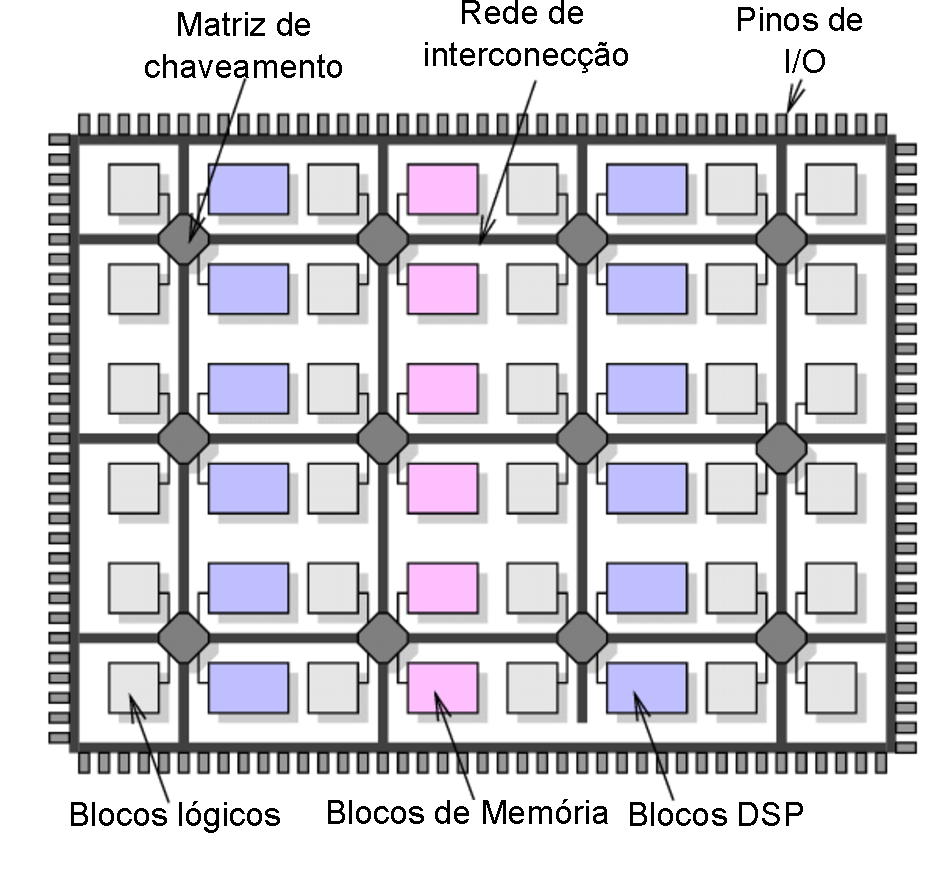
\includegraphics[width=0.65\linewidth]{figs/FPGA/FPGA.pdf}
    \caption{Arquitetura interna de um FPGA. Adaptado de \citeonline{langhammer2014design}}
    \label{fig:FPGA_internal_architeture}
\end{figure}

De modo geral, a arquitetura de um FPGA moderno pode ser compreendida como um arranjo matricial de elementos lógicos, conectados por uma rede de roteamento programável e complementados por blocos dedicados de memória, processamento aritmético e comunicação Figura~\ref{fig:FPGA_internal_architeture}. Essa organização possibilita a construção de circuitos personalizados, capazes de operar de forma determinística e com latência previsível — características essenciais em sistemas embarcados e aplicações de tempo real.

Os principais componentes que compõem essa arquitetura, enfatizando suas funções e a forma como interagem na implementação de sistemas digitais \mbox{complexos são listado a seguir:}

\begin{itemize}
	\item \textbf{Blocos Lógicos Configuráveis (CLBs / Logic Elements)}
	Cada bloco lógico geralmente contém uma \textit{Look-Up Table, LU)}, \textit{flip-flops} (registradores) e lógica de seleção (multiplexadores). As LUTs são usadas para implementar funções lógicas arbitrárias (até uma certa \textit{fan-in}). Os \textit{flip-flops} armazenam estado, e a lógica de interconexão dentro do bloco permite configuração de lógica combinacional ou sequencial.
	
	\item \textbf{Rede de Interconexão Programável}
	Os blocos lógicos são conectados por uma malha (ou rede) de trilhas metálicas (vias, linhas horizontais e verticais) e \textit{switches} programáveis (\textit{crossbars}, multiplexadores, \textit{buffers}). Essa rede determina como os sinais trafegam entre blocos. O desafio de roteamento (satisfazer todas as conexões com restrições de temporização\textit{timing}) é crítico para o desempenho final.
	
	\item \textbf{Blocos de Entrada/Saída (I/O Blocks)}
	Permitem a interface com sinais externos (barramentos, memórias externas, sensores, periféricos). Tipicamente suportam múltiplos padrões de tensão e protocolos (por exemplo, LVDS, PCIe, DDR, \mbox{interfaces de alta velocidade).}
	
	\item \textbf{Blocos de Memória (BRAM / Block RAM)}
	Memórias internas, distribuídas dentro do FPGA, oferecem armazenamento rápido e local para dados intermediários, buffers, tabelas etc. São mais rápidas e eficientes que acessar memória externa.
	
	\item \textbf{Blocos DSP (DSP Slices)}
	Otimizados para operações aritméticas, especialmente multiplicações, multiplicações acumuladas e outras operações de ponto fixo ou ponto flutuante limitada. Permitem acelerar operações pesadas tipicamente usadas em filtros, transformadas, redes neurais etc.
	
	\item \textbf{Transceptores Seriais de Alta Velocidade}
	Alguns FPGAs integram transceptores seriais (links de alta velocidade) que permitem comunicação externa (por exemplo, PCIe, Ethernet de alta velocidade, canais seriais até várias \mbox{dezenas ou centenas de Gbps).}
	
	\item \textbf{Sistemas em Chip (SoC) Integrados}
	Muitos FPGAs modernos incorporam processadores (por exemplo, ARM Cortex, RISC-V) no mesmo chip, compartilhando recursos com a lógica reconfigurável. Isso possibilita uma arquitetura heterogênea: parte do sistema roda em software (no processador), outra parte em lógica personalizada (hardware), com comunicação interna eficiente entre os dois.
	
	\item \textbf{Suporte a Recursos Avançados}
	FPGAs mais recentes podem possuir recursos como reconfiguração parcial dinâmica, blocos de lógica adaptativa (motores de IA, blocos especializados), interconexão multi-DIE (em FPGAs grandes), e suporte a lógica adaptativa para redes neurais (por exemplo, motores de multiplicação de baixa precisão, compressão, suporte a esparsidade, etc.).
\end{itemize}

%A Tabela ~\ref{tab:arquitetura_fpga}, detalha os principais componentes que compõem essa arquitetura, enfatizando suas funções e a forma como interagem na implementação de sistemas digitais complexos:

%\begin{table}[H]
%\centering
%\caption{Principais componentes da arquitetura interna de um FPGA e suas respectivas funções.}
%\label{tab:arquitetura_fpga}
%\renewcommand{\arraystretch}{1.3}
%\resizebox{\textwidth}{!}{%
%\begin{tabular}{p{4cm} p{12cm}}
%\hline
%\textbf{Componente} & \textbf{Descrição e Função Principal} \\ \hline
%
%\textbf{Blocos Lógicos Configuráveis (CLBs / Logic Elements)} &
%Unidades fundamentais de processamento do FPGA, a Figura~\ref{fig:FPGA_CBL} apresente um CBL ilustrativo. Cada CLB contém uma ou mais \textit{Look-Up Tables} (LUTs), registradores (flip-flops) e multiplexadores, permitindo implementar funções lógicas combinacionais ou sequenciais. As LUTs armazenam tabelas de verdade de até $2^n$ entradas, enquanto os flip-flops permitem o armazenamento de estado e sincronização com o clock global. \\ \hline
%
%\textbf{Rede de Interconexão Programável} &
%Responsável por conectar os CLBs, BRAMs, DSPs e demais blocos através de trilhas metálicas horizontais e verticais, controladas por comutadores programáveis (\textit{switch boxes} e \textit{connection boxes}). Essa rede define o fluxo de dados e é determinante para o desempenho do circuito, sendo o processo de roteamento e temporização (timing closure) um dos desafios centrais do projeto em FPGA. \\ \hline
%
%\textbf{Blocos de Entrada/Saída (I/O Blocks)} &
%Interfaceiam o FPGA com dispositivos externos, permitindo comunicação com memórias, barramentos, sensores e periféricos. Suportam múltiplos padrões elétricos (LVCMOS, LVDS, SSTL) e protocolos de alta velocidade, como PCIe, DDR e Ethernet, além de oferecer recursos de calibração e proteção elétrica. \\ \hline
%
%\textbf{Blocos de Memória (BRAM / Block RAM)} &
%Memórias estáticas internas distribuídas na matriz lógica, utilizadas para armazenamento local de dados, buffers de transmissão, tabelas de coeficientes e pesos de redes neurais. Possuem latência extremamente baixa e são configuráveis em diferentes larguras e profundidades. \\ \hline
%
%\textbf{Blocos DSP (DSP Slices)} &
%Unidades aritméticas dedicadas a operações de multiplicação, soma acumulada (MAC) e cálculos de ponto fixo ou ponto flutuante reduzido. São essenciais em tarefas de alto desempenho, como filtragem digital (FIR/IIR), transformadas rápidas (FFT) e aceleração de camadas convolucionais em redes neurais. \\ \hline
%
%\textbf{Transceptores Seriais de Alta Velocidade} &
%Módulos especializados que permitem comunicação externa por meio de canais seriais de alta taxa de transferência (até centenas de Gbps), utilizados em protocolos como PCIe, SATA, Ethernet e JESD204. Possuem circuitos de equalização e controle de clock para integridade de sinal. \\ \hline
%
%\textbf{Sistemas em Chip (SoC) Integrados} &
%FPGAs modernos podem incluir processadores embutidos (ex.: ARM Cortex-A9, RISC-V), formando uma arquitetura heterogênea. Essa integração permite executar parte do sistema em software e parte em hardware, com comunicação interna de alta largura de banda por barramentos AXI (\textit{Advanced eXtensible Interface}). \\ \hline
%
%\textbf{Recursos Avançados e Funcionalidades Adicionais} &
%Modelos recentes incorporam reconfiguração parcial dinâmica (\textit{Partial Reconfiguration}), blocos de lógica adaptativa (AI Engines) e interconexão multi-die (em dispositivos de grande porte). Tais recursos suportam otimizações específicas para aprendizado de máquina, como operações com baixa precisão, compressão de pesos e suporte a sparsidade. \\ \hline
%\end{tabular}}
%\end{table}

\begin{figure}[H]
    \centering
    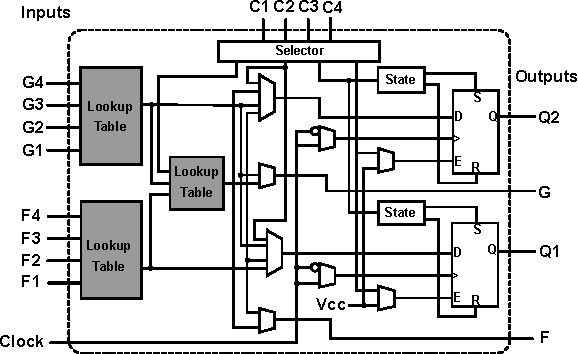
\includegraphics[width=0.8\linewidth]{figs/FPGA/CBL.pdf}
    \caption{Imagem ilustrativa de um \textit{CBL}. Adaptado de \citeonline{genera_technologies_fpga}}
    \label{fig:FPGA_CBL}
\end{figure}

Além disso, o modelo de temporização, timing, nos FPGAs é fundamental: cada sinal tem um caminho entre flip-flops, com restrições de tempo (\textit{setup}, \textit{hold}), e o roteamento de pistas e \textit{buffers} intermediários afetam a latência e taxa máxima de \textit{clock} \mbox{que pode ser alcançada.}

% \subsection*{Fluxo de Desenvolvimento com FPGA}

% Um mapeamento mais detalhado do fluxo de desenvolvimento FPGA típico, com ênfase em aplicações de IA, pode ser descrito da seguinte forma:

% \begin{enumerate}
% \item \textbf{Definição do algoritmo / modelo}
% No caso de IA, inicia-se com o projeto ou escolha da rede neural (topologia, número de camadas, tipo de ativação, quantização, compressão etc.).

% \item \textbf{Quantização / otimização de modelo}
% Para reduzir custo de hardware e latência, frequentemente aplica-se quantização (redução da largura de bits dos pesos e ativações), poda (pruning), compressão esparsa, fatoração ou aproximação de operações.

% \item \textbf{Descrição em HDL ou HLS (High-Level Synthesis)}
% A rede otimizada é então implementada usando linguagens de descrição de hardware (VHDL, Verilog) ou por meio de ferramentas HLS que compilam descrições em C/C++/OpenCL para hardware. As ferramentas HLS permitem abstração mais alta, mas exigem atenção à qualidade do hardware gerado (área, latência, paralelismo).

% \item \textbf{Síntese Lógica}
% A ferramenta converte a descrição de alto nível em uma rede de portas lógicas (LUTs, flip-flops, blocos DSP) lógicas equivalentes.

% \item \textbf{Implementação (Place & Route)}
% O mapeamento lógico é alocado em CLBs, rotas são calculadas pela ferramenta de roteamento, e as interconexões entre blocos são estabelecidas. Aqui ocorrem problemas de congestionamento e restrições de tempo.

% \item \textbf{Análise de Tempo e Ajustes}
% Após roteamento, é feita análise estática de tempo para verificar se os caminhos críticos atendem às restrições de clock. Caso contrário, ajusta-se pipeline, duplicação de lógica, re-rastro, bufferização, restrições de roteamento etc.

% \item \textbf{Geração do Bitstream e Programação}
% O arquivo de configuração (bitstream) é gerado e carregado no FPGA, configurando a interconexão e lógica conforme o design projetado.

% \item \textbf{Verificação / Validação / Testes em Hardware}
% Finalmente, testa-se o circuito configurado (validação funcional, testes de desempenho, consumo, latência, estabilidade).

% \item \textbf{Iterações / Otimizações}
% Muitas vezes, múltiplas iterações são necessárias: ajustes no modelo, re-quantização, pipeline mais fino, divisão em blocos, paralelismo, balanceamento de carga, uso de memória local etc.

% \end{enumerate}

\subsection*{Fluxo de Desenvolvimento com FPGA}

O fluxo de desenvolvimento em FPGAs segue uma sequência bem definida de etapas, que vão desde a concepção do algoritmo até a implementação e validação física do projeto no dispositivo. Esse processo é especialmente relevante em aplicações de Inteligência Artificial (IA) e aprendizado profundo, nas quais o equilíbrio entre desempenho, consumo e utilização de recursos é determinante para a viabilidade do sistema.

O fluxo de desenvolvimento em FPGA, com ênfase em aplicações de Inteligência Artificial, pode ser descrito como uma sequência de etapas encadeadas, que vão desde a definição conceitual do modelo até a validação em hardware e as \mbox{iterações finais de otimização.}

Inicialmente, na \textbf{definição do algoritmo ou modelo}, estabelece-se o comportamento desejado do sistema digital. Em aplicações de IA, essa etapa envolve a escolha ou o projeto de uma arquitetura de rede neural adequada (por exemplo, definição do número de camadas, tipos de ativação, organização MLP e tamanho dos filtros), considerando simultaneamente requisitos de precisão, latência, uso de recursos e complexidade computacional. Trata-se de uma fase predominantemente algorítmica, na qual ainda não se impõem, de forma explícita, as restrições do dispositivo FPGA alvo.

Em seguida, ocorre a \textbf{quantização e otimização do modelo}, cujo objetivo é reduzir o custo computacional e a demanda de recursos de hardware, preservando, tanto quanto possível, a acurácia do modelo. Técnicas como quantização de pesos e ativações (redução da largura de bits), poda (\textit{pruning}), compressão esparsa e fatoração de matrizes são empregadas para diminuir o número de operações e o volume de dados trafegados. Essa etapa é particularmente crítica em FPGAs, dado que LUTs, blocos DSP e BRAMs são recursos finitos e precisam ser utilizados de forma eficiente.

A arquitetura já otimizada é então traduzida para uma \textbf{descrição em HDL ou HLS (High-Level Synthesis)}. Nessa fase, o projeto é implementado em linguagens de descrição de hardware tradicionais, como VHDL ou Verilog, ou em linguagens de mais alto nível (C/C++/OpenCL) que serão sintetizadas por ferramentas de HLS. Embora o HLS facilite o desenvolvimento e aumente o nível de abstração, ele exige uma análise cuidadosa da qualidade do hardware gerado, sobretudo no que diz respeito à área ocupada, ao grau de paralelismo explorado e à latência dos caminhos críticos.

A etapa seguinte corresponde à \textbf{sintese lógica}, na qual a descrição funcional é convertida em uma rede lógica equivalente composta por LUTs, flip-flops, blocos DSP e memórias internas (BRAMs) do FPGA. As ferramentas de síntese aplicam otimizações de lógica booleana, realizam o mapeamento para os recursos específicos do dispositivo e geram uma representação intermediária que servirá de base para o \mbox{processo de implementação física.}

Concluída a síntese, procede-se à \textbf{implementação física (\textit{place \& route})}. Nessa fase, os elementos lógicos são posicionados na matriz do FPGA (\textit{placement}) e as conexões elétricas entre eles são estabelecidas (\textit{routing}). A forma como os blocos (CLBs, DSPs, BRAMs) são distribuídos e interligados impacta diretamente a frequência máxima de operação e o consumo de energia. Congestionamentos na rede de interconexão ou rotas excessivamente longas podem impedir o cumprimento das metas de \mbox{temporização definidas no projeto.}

Após o roteamento, realiza-se a \textbf{análise de tempo e o \textit{timing closure}}. Por meio de análise estática de temporização, verificam-se as restrições de \textit{setup} e \textit{hold} em todos os caminhos relevantes. Caso os caminhos críticos excedam o período de clock especificado, torna-se necessário aplicar técnicas de otimização, tais como inserção de estágios adicionais de pipeline, replicação de lógica, refinamento de restrições ou reorganização de blocos. O objetivo é garantir que o design opere de forma confiável na frequência alvo.

Uma vez satisfeitas as restrições de temporização, procede-se à \textbf{geração do bitstream e programação do dispositivo}. A configuração final é codificada em um arquivo de bits (\textit{bitstream}) que descreve completamente a interconexão e o comportamento interno do FPGA. Esse arquivo é então carregado no dispositivo por meio de interfaces apropriadas (como JTAG, SPI ou USB), configurando-o conforme o projeto desenvolvido.

Na sequência, ocorre a fase de \textbf{verificação e testes em hardware}, em que o design é validado fisicamente no FPGA. São realizados testes funcionais, medições de desempenho, análise de estabilidade e avaliação do consumo energético. Em aplicações de IA, é usual executar a inferência diretamente no hardware, comparando-se a acurácia e o tempo de resposta com aqueles obtidos em simulação ou em plataformas de referência (CPU/GPU), especialmente após a quantização e outras otimizações.

Por fim, o processo raramente se encerra em uma única passagem. Assim, fala-se em \textbf{iterações e otimizações finais}, nas quais o projetista retorna a etapas anteriores para ajustar parâmetros, refinar o pipeline, melhorar o paralelismo, reorganizar \textit{buffers} de memória local e equilibrar a utilização de recursos lógicos e de comunicação. Esse ciclo iterativo é característico do desenvolvimento em FPGA e permite gradualmente aproximar o projeto dos requisitos almejados de latência, \textit{throughput}, \mbox{consumo de energia e área ocupada.}


%O fluxo de desenvolvimento em FPGAs segue uma sequência bem definida de etapas, que vão desde a concepção do algoritmo até a implementação e validação física do projeto no dispositivo. Esse processo, representado de forma resumida na Tabela~\ref{tab:fluxo_fpga}, é especialmente relevante em aplicações de Inteligência Artificial (IA) e aprendizado profundo, nas quais o equilíbrio entre desempenho, consumo e utilização de recursos é determinante para a viabilidade do sistema.

%\begin{table}[H]
%\centering
%\caption{Etapas típicas do fluxo de desenvolvimento em FPGA, com ênfase em aplicações de Inteligência Artificial.}
%\label{tab:fluxo_fpga}
%\renewcommand{\arraystretch}{1.3}
%\resizebox{\textwidth}{!}{%
%\begin{tabular}{p{4cm} p{12cm}}
%\hline
%\textbf{Etapa} & \textbf{Descrição e Objetivos Principais} \\ \hline
%
%\textbf{1. Definição do Algoritmo ou Modelo} &
%Corresponde à etapa inicial do projeto, na qual se define o comportamento desejado do sistema digital. Em aplicações de IA, envolve a escolha ou o desenvolvimento de uma arquitetura de rede neural (número de camadas, tipo de ativação, estrutura MLP, etc.), levando em conta requisitos de precisão, latência e complexidade. \\ \hline
%
%\textbf{2. Quantização e Otimização do Modelo} &
%Visa reduzir a complexidade computacional e o consumo de recursos do FPGA. Técnicas como quantização (redução da largura de bits de pesos e ativações), poda (\textit{pruning}), compressão esparsa e fatoração de matrizes são aplicadas para otimizar o desempenho e minimizar a latência sem comprometer a acurácia do modelo. \\ \hline
%
%\textbf{3. Descrição em HDL ou HLS (High-Level Synthesis)} &
%A arquitetura otimizada é implementada em uma linguagem de descrição de hardware (VHDL, Verilog) ou em linguagens de alto nível (C/C++/OpenCL) compiladas por ferramentas de \textit{High-Level Synthesis}. O HLS facilita o desenvolvimento, mas requer análise criteriosa da qualidade do hardware gerado, especialmente em termos de área, paralelismo e latência. \\ \hline
%
%\textbf{4. Síntese Lógica} &
%Converte a descrição funcional em uma rede lógica equivalente composta por LUTs, flip-flops, blocos DSP e BRAMs. Nessa etapa são aplicadas otimizações automáticas de lógica booleana e mapeamento de recursos específicos do dispositivo alvo. \\ \hline
%
%\textbf{5. Implementação (Place \& Route)} &
%Os elementos lógicos são fisicamente mapeados na matriz do FPGA. O processo de \textit{placement} define a alocação espacial dos blocos (CLBs, DSPs, BRAMs), enquanto o \textit{routing} estabelece as conexões elétricas entre eles. Essa fase é crítica para o desempenho, pois o congestionamento ou roteamento inadequado pode limitar a frequência máxima de operação. \\ \hline
%
%\textbf{6. Análise de Tempo e Ajustes (Timing Closure)} &
%Após o roteamento, é realizada a análise estática de tempo, que verifica o cumprimento das restrições de temporização (\textit{setup} e \textit{hold}). Caso os caminhos críticos ultrapassem o período de clock, aplicam-se técnicas de otimização, como inserção de pipeline, replicação de lógica e ajustes de restrições. \\ \hline
%
%\textbf{7. Geração do Bitstream e Programação} &
%A configuração final é traduzida em um arquivo de bits (\textit{bitstream}), responsável por definir a interconexão e o comportamento interno do FPGA. Esse arquivo é então carregado no dispositivo por meio de interfaces JTAG, SPI ou USB, configurando-o conforme o projeto desenvolvido. \\ \hline
%
%\textbf{8. Verificação e Testes em Hardware} &
%Nesta fase, o design é validado fisicamente. São realizados testes de funcionalidade, desempenho, estabilidade e consumo energético. Em projetos de IA, é comum realizar inferência direta no FPGA para medir a precisão do modelo após quantização e integração. \\ \hline
%
%\textbf{9. Iterações e Otimizações Finais} &
%O ciclo de desenvolvimento raramente é linear. Geralmente, diversas iterações são necessárias para ajustar parâmetros, refinar o pipeline, melhorar o paralelismo, reorganizar buffers de memória local e equilibrar a utilização de recursos lógicos e de comunicação. \\ \hline
%\end{tabular}}
%\end{table}

O processo de desenvolvimento e otimização de projetos em FPGA pode ser sintetizado na Figura~\ref{fig:FluxoDesenvolvimentoFPGA}, que apresenta, de forma esquemática, o ciclo completo desde a definição inicial do algoritmo até a validação em hardware. Esse fluxo evidencia o caráter iterativo do desenvolvimento em dispositivos reconfiguráveis, no qual a cada etapa — da modelagem à implementação física — o projetista deve buscar o equilíbrio entre desempenho, \mbox{consumo e utilização de recursos lógicos.}

\begin{figure}[H]
    \centering
    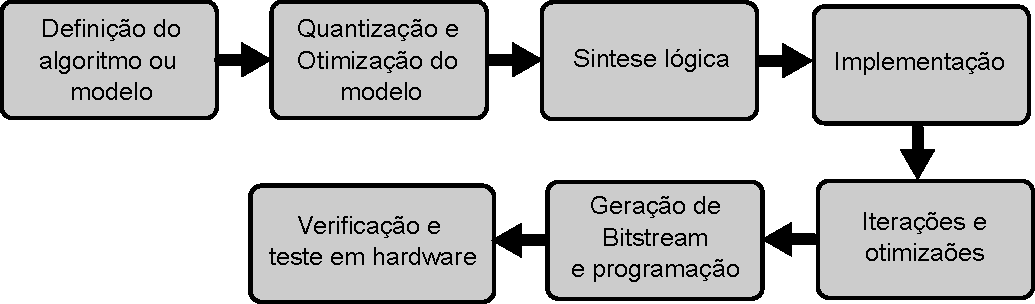
\includegraphics[width=0.8\linewidth]{figs/FPGA/FluxoOtimização.pdf}
    \caption{Fluxo de desenvolvimento e otimização de projetos em FPGA. O autor.}
    \label{fig:FluxoDesenvolvimentoFPGA}
\end{figure}

A Figura~\ref{fig:FluxoDesenvolvimentoFPGA} destaca a sequência típica de etapas: inicia-se pela definição do modelo ou algoritmo, seguida pela quantização e otimização, que reduzem a complexidade computacional. Na sequência, a descrição em HDL ou por meio de ferramentas de HLS permite traduzir o comportamento algorítmico em lógica digital reconfigurável. As fases de síntese e \textit{place \& route} realizam o mapeamento físico do projeto sobre os blocos lógicos e interconexões do FPGA, seguidas da análise de temporização, responsável por assegurar que todas as restrições de tempo de propagação sejam satisfeitas. Por fim, ocorre a geração do \textit{bitstream}, etapa na qual o projeto é convertido em um arquivo de configuração e carregado no dispositivo para verificação e validação funcional.

Ao final do ciclo, ajustes e otimizações adicionais são frequentemente necessários, refletindo o caráter experimental e aprimorável do processo. Essa natureza iterativa é fundamental em aplicações de Inteligência Artificial, nas quais a eficiência do hardware depende diretamente do grau de paralelismo, da largura de barramento e da arquitetura da rede neural mapeada no FPGA.


O sucesso do projeto depende da integração eficiente entre as etapas de síntese, implementação e análise de tempo. Pequenas variações no roteamento ou na granularidade do paralelismo podem impactar significativamente a taxa máxima de \textit{clock} e o consumo energético do sistema, sobretudo em aplicações de aprendizado profundo com restrições de latência e \textit{throughput}.

No contexto de aplicações de Inteligência Artificial, algumas etapas do fluxo de desenvolvimento em FPGA exigem atenção especial para garantir eficiência e desempenho. O \textit{quantization-aware training}, por exemplo, permite que o modelo seja treinado levando em consideração os efeitos da quantização, preservando a acurácia mesmo com representações de baixa precisão. O mapeamento eficiente de multiplicações binárias ou quantizadas — frequentemente implementadas em blocos DSP — é essencial para maximizar o paralelismo e reduzir o consumo de área lógica. Da mesma forma, o suporte à ``esparsidade'' de valores nulos e a utilização otimizada de memórias locais (BRAM e URAM) são fatores decisivos para minimizar a dependência de acessos à memória externa, os quais representam um dos principais gargalos de desempenho em arquiteturas reconfiguráveis.  

Essas estratégias de otimização, quando bem empregadas, tornam os FPGAs especialmente adequados para aplicações embarcadas de IA e aprendizado profundo, nas quais o equilíbrio entre consumo energético, latência e throughput é determinante para a viabilidade prática do sistema.

% A subseção a seguir apresenta uma análise comparativa das principais vantagens e limitações desses dispositivos, considerando seu uso em aceleração de algoritmos de inteligência artificial.

%\subsection*{Vantagens e Desvantagens dos FPGAs (na perspectiva de IA)}
%
%O uso de FPGAs em aplicações de Inteligência Artificial apresenta um conjunto de vantagens que os torna particularmente atrativos para a implementação de algoritmos de aprendizado profundo e de processamento de sinais em tempo real. Em especial, destacam-se aspectos como flexibilidade de reconfiguração, exploração de paralelismo em nível de hardware e potencial de eficiência energética em cenários de inferência embarcada e de borda, \textit{edge computing}. A seguir, são sintetizados alguns dos principais pontos fortes associados a essa tecnologia:
%
%\begin{itemize}
%	\item \textbf{Reconfigurabilidade e adaptabilidade:} possibilita modificar o hardware após a fabricação, permitindo ajustar a arquitetura à medida que o modelo de IA ou os requisitos do sistema evoluem, sem necessidade de projetar um novo circuito integrado dedicado.
%	
%	\item \textbf{Paralelismo massivo:} os recursos lógicos internos permitem a execução simultânea de múltiplas operações, explorando de forma direta o paralelismo intrínseco de redes neurais, filtros convolucionais e demais blocos de processamento distribuído.
%	
%	\item \textbf{Baixa latência e previsibilidade temporal:} a ausência de camadas intermediárias de software e de sistemas operacionais complexos favorece um comportamento determinístico, com latência reduzida e previsível — característica essencial em aplicações em tempo real e em sistemas de controle crítico.
%	
%	\item \textbf{Eficiência energética:} quando adequadamente otimizados, projetos em FPGA podem alcançar maior eficiência em termos de operações por joule (ops/J) do que soluções baseadas exclusivamente em GPU, especialmente em cenários de inferência local e dispositivos de borda.
%	
%	\item \textbf{Customização de precisão:} o suporte à implementação de operações com diferentes larguras de palavra (por exemplo, formatos binários, ternários ou de 4–8 bits) permite ajustar o uso de recursos de hardware de acordo com a tolerância do modelo à quantização, equilibrando acurácia e custo computacional.
%	
%	\item \textbf{Integração de funções heterogêneas:} em um único chip, é possível combinar blocos de controle, interfaces de comunicação, módulos de pré-processamento e pós-processamento de sinais, reduzindo a latência de comunicação entre etapas e o consumo global do sistema.
%\end{itemize}


%O uso de FPGAs em aplicações de Inteligência Artificial apresenta um conjunto de vantagens que os tornam altamente atrativos para a implementação de algoritmos de aprendizado profundo e processamento de sinais em tempo real. A Tabela~\ref{tab:fpga_vantagens} sintetiza os principais aspectos positivos observados na literatura e na prática industrial, destacando sua flexibilidade, paralelismo e eficiência energética — fatores determinantes para aplicações embarcadas e de borda (\textit{edge computing}).
%
%\begin{table}[H]
%\centering
%\caption{Principais vantagens dos FPGAs em aplicações de Inteligência Artificial.}
%\label{tab:fpga_vantagens}
%\renewcommand{\arraystretch}{1.3}
%\resizebox{\textwidth}{!}{%
%\begin{tabular}{p{4cm} p{12cm}}
%\hline
%\textbf{Vantagem} & \textbf{Descrição} \\ \hline
%
%\textbf{Reconfigurabilidade e adaptabilidade} &
%Permite modificar o hardware após a fabricação, possibilitando ajustes à medida que o modelo ou os requisitos do sistema evoluem, sem a necessidade de novos projetos físicos. \\ \hline
%
%\textbf{Paralelismo massivo} &
%Os recursos lógicos permitem a execução simultânea de múltiplas operações, explorando o paralelismo intrínseco de redes neurais e filtros convolucionais. \\ \hline
%
%\textbf{Baixa latência e previsibilidade temporal} &
%A ausência de camadas intermediárias de software garante processamento determinístico, ideal para aplicações em tempo real e controle crítico. \\ \hline
%
%\textbf{Eficiência energética} &
%Projetos bem otimizados em FPGA podem atingir maior eficiência em operações por joule (ops/J) do que GPUs, especialmente em aplicações de inferência local e dispositivos de borda. \\ \hline
%
%\textbf{Customização de precisão} &
%Suporte à implementação de operações com diferentes larguras de palavra (binária, ternária, 4–8 bits), ajustando o consumo de recursos conforme a tolerância do modelo à quantização. \\ \hline
%
%\textbf{Integração de funções heterogêneas} &
%Permite integrar, em um único chip, blocos de controle, interfaces de comunicação, pré-processamento e pós-processamento de sinais, reduzindo latência e consumo. \\ \hline
%\end{tabular}}
%\end{table}

%Apesar de seus benefícios, o uso de FPGAs em aplicações de Inteligência Artificial também apresenta limitações e desafios que precisam ser cuidadosamente considerados no processo de projeto. Em particular, destacam-se restrições de recursos físicos, maior complexidade de desenvolvimento e um ciclo de projeto mais longo quando comparado a plataformas mais convencionais. A seguir, são sintetizados alguns dos principais pontos críticos associados a essa tecnologia:
%
%\begin{itemize}
%	\item \textbf{Recursos limitados:} a quantidade de blocos lógicos, unidades DSP e memórias internas (BRAMs) disponível em um FPGA é finita. Redes neurais de grande porte ou modelos com elevado número de parâmetros podem exceder a capacidade do dispositivo, exigindo estratégias adicionais de quantização, poda ou \mbox{particionamento do modelo.}
%	
%	\item \textbf{Complexidade de projeto:} o desenvolvimento em FPGA demanda domínio de linguagens de descrição de hardware (como VHDL e Verilog) ou de fluxos baseados em \textit{High-Level Synthesis}, além de conhecimento em síntese lógica, fechamento de temporização e otimização de desempenho. Esse conjunto de competências torna a curva de aprendizado mais íngreme quando comparado a frameworks de alto nível em CPU ou GPU.
%	
%	\item \textbf{Desempenho inferior a ASICs dedicados:} embora ofereçam flexibilidade e reconfigurabilidade, FPGAs não alcançam, em geral, a mesma densidade lógica nem a mesma eficiência energética de circuitos integrados de aplicação específica (ASICs) projetados sob medida para uma determinada rede ou tarefa.
%	
%	\item \textbf{Consumo em uso contínuo:} em aplicações de longa duração e alta taxa de utilização, o consumo energético total pode superar o de soluções especializadas ou de chips dedicados, sobretudo quando o projeto não explora plenamente recursos de desligamento parcial, \textit{clock gating} ou outras técnicas de economia de energia.
%	
%	\item \textbf{Tempo de desenvolvimento elevado:} etapas como implementação física, \textit{place \& route}, fechamento de temporização, \textit{timing closure}, balanceamento de pipeline e ajuste fino de restrições podem demandar múltiplas iterações, aumentando significativamente o tempo total de desenvolvimento em comparação com arquiteturas puramente de software.
%	
%	\item \textbf{Gargalos de memória externa:} o acesso frequente à memória DRAM externa pode introduzir latência adicional e elevar o consumo de energia. Isso exige estratégias cuidadosas de uso de memória local (BRAMs, buffers e caches) e de reutilização de dados para evitar que a banda de memória se torne o \mbox{principal limitante do desempenho.}
%	
%	\item \textbf{Desafios de quantização e precisão:} a necessidade de reduzir a largura de palavra (por exemplo, para 8, 4 ou até 1–2 bits) a fim de caber no FPGA pode conduzir à degradação da acurácia do modelo. Encontrar o equilíbrio entre custo de hardware e desempenho preditivo é uma tarefa não trivial, frequentemente exigindo técnicas de \textit{quantization-aware training} e experimentação extensiva.
%\end{itemize}


%Apesar de seus benefícios, o uso de FPGAs também apresenta limitações que devem ser consideradas durante o processo de desenvolvimento. Conforme resumido na Tabela~\ref{tab:fpga_desvantagens}, os principais desafios envolvem restrições de recursos físicos, complexidade de projeto, e tempo de desenvolvimento — fatores que demandam conhecimento especializado em arquitetura digital e ferramentas de síntese.
%
%\begin{table}[H]
%\centering
%\caption{Principais desvantagens e desafios no uso de FPGAs para aplicações de IA.}
%\label{tab:fpga_desvantagens}
%\renewcommand{\arraystretch}{1.3}
%\resizebox{\textwidth}{!}{%
%\begin{tabular}{p{4cm} p{12cm}}
%\hline
%\textbf{Desvantagem} & \textbf{Descrição} \\ \hline
%
%\textbf{Recursos limitados} &
%A quantidade de blocos lógicos, DSPs e memórias internas é finita; redes neurais de grande porte podem exceder a capacidade disponível. \\ \hline
%
%\textbf{Complexidade de projeto} &
%O desenvolvimento requer domínio de linguagens de descrição de hardware (VHDL, Verilog) e ferramentas de síntese, além de experiência com restrições temporais e otimização de performance. \\ \hline
%
%\textbf{Desempenho inferior a ASICs} &
%Embora flexível, o FPGA não atinge a mesma densidade lógica nem a eficiência energética de um ASIC dedicado para a mesma aplicação. \\ \hline
%
%\textbf{Consumo em uso contínuo} &
%Para tarefas de longa duração, o consumo energético pode superar soluções otimizadas ou chips dedicados. \\ \hline
%
%\textbf{Tempo de desenvolvimento elevado} &
%Etapas como roteamento, fechamento de temporização (\textit{timing closure}) e balanceamento de pipeline aumentam significativamente o tempo de iteração. \\ \hline
%
%\textbf{Gargalos de memória externa} &
%O acesso à memória DRAM externa pode introduzir latência e elevar o consumo de energia, exigindo estratégias de uso eficiente da memória local. \\ \hline
%
%\textbf{Desafios de quantização e precisão} &
%A redução excessiva da precisão pode degradar a acurácia do modelo; equilibrar custo de hardware e desempenho é uma tarefa complexa. \\ \hline
%\end{tabular}}
%\end{table}

%Diante desse conjunto de vantagens e limitações, o uso de FPGAs em aplicações de Inteligência Artificial caracteriza-se por um claro compromisso entre desempenho, flexibilidade e complexidade de desenvolvimento. 
%
%Por um lado, a possibilidade de explorar paralelismo em nível de hardware, customizar a precisão numérica e integrar, em um único dispositivo, funções de aquisição, processamento e decisão torna os FPGAs particularmente atraentes para sistemas de monitoramento em tempo real baseados em aprendizado de máquina. Por outro, a necessidade de lidar com recursos restritos, fluxos de projeto mais complexos e desafios de quantização demanda uma fase prévia de estudo e modelagem cuidadosa antes de se partir para a implementação física. 
%
%Nesse contexto, o presente trabalho concentra-se em um \textit{estudo de viabilidade} por meio de simulação de uma arquitetura baseada em rede MLP embarcada em FPGA, utilizando o framework FINN como ferramenta de apoio ao mapeamento em hardware.
%



%O objetivo é compreender, de forma sistemática, como os trade-offs entre acurácia, latência e uso de recursos podem ser equilibrados em um cenário de detecção de cavitação por emissão acústica, fornecendo subsídios técnicos para futuras etapas de prototipagem e implementação real.


\subsection{Otimização de IA em FPGAs: técnicas, desafios e tendências}

Para que redes neurais sejam mapeadas de forma eficiente em FPGAs, é necessário aplicar um conjunto de técnicas de otimização que atuam simultaneamente sobre a arquitetura do modelo, a representação numérica dos dados e a própria organização interna do hardware, garantindo assim um melhor aproveitamento dos recursos disponíveis.

Em linhas gerais, essas estratégias buscam reduzir latência, consumo de energia e uso de área lógica, preservando, tanto quanto possível, a acurácia do modelo. A seguir, são apresentadas algumas das principais abordagens relatadas na literatura recente para aceleração de redes neurais em FPGAs:

\begin{itemize}
	\item \textbf{Quantização:} consiste em reduzir a largura de bits de pesos e ativações (por exemplo, para 8, 4, 2 ou mesmo 1 bit), diminuindo o uso de DSPs e de memória interna. Quando combinada com treinamento ciente de quantização (\textit{quantization-aware training}), essa técnica permite obter modelos mais compactos com perda limitada de desempenho, sendo uma das bases de muitos fluxos de implementação em FPGA.
	
	\item \textbf{Poda e exploração de esparsidade:} remove conexões cujos pesos são próximos de zero, reduzindo o número de operações aritméticas e acessos à memória. Para que o ganho seja efetivo em hardware, é necessário que a arquitetura seja projetada para explorar essa esparsidade de maneira estruturada, evitando \textit{overheads} de controle que anulam o benefício.
	
	\item \textbf{Fusão de camadas e compressão de operadores:} integra operações que, tradicionalmente, seriam tratadas de forma separada — como convolução, ativação e \textit{pooling}, em um único bloco funcional. Essa fusão diminui o tráfego de dados entre módulos, reduz a lógica de interconexão e pode simplificar o roteamento e o controle do fluxo de informações.
	
	\item \textbf{Fatoração e decomposição de operações:} convoluções maiores (como filtros \(3\times3\) ou \(5\times5\)) podem ser decompostas em operações menores ou sequenciais, de forma a economizar recursos lógicos e facilitar o fechamento de temporização. Em alguns casos, decomposições separáveis (espacial ou em canais) permitem diminuir significativamente o custo computacional.
	
	\item \textbf{Pipeline e paralelismo fino:} divide-se o processamento em múltiplos estágios de pipeline, permitindo que diferentes amostras ou partes do cálculo sejam processadas simultaneamente em fases distintas. Esse paralelismo fino, típico de arquiteturas \textit{streaming}, contribui para manter o \textit{throughput} elevado com latência de \mbox{cada estágio controlada.}
	
	\item \textbf{Uso eficiente de memória local:} maximiza-se o aproveitamento de BRAMs, URAMs e \textit{buffers} internos para reduzir a dependência da DRAM externa. Estratégias de \textit{tiling}, reutilização de dados e armazenamento em janelas deslizantes são fundamentais para evitar que o gargalo de memória se torne o \mbox{principal limitante do desempenho.}
	
	\item \textbf{Compressão e codificação de pesos:} emprega técnicas como compressão \textit{run-length} e codificação de comprimento variável para reduzir o tamanho do modelo e o volume de dados transferidos. Em combinação com sparsidade, essa abordagem contribui para diminuir a largura de banda necessária entre memória e \mbox{unidades de processamento.}
	
	\item \textbf{Aritmética aproximada:} substitui operações exatas por variantes aproximadas (por exemplo, somadores e multiplicadores aproximados), com menor custo de implementação. Desde que o erro introduzido permaneça dentro de limites aceitáveis para a aplicação, é possível reduzir significativamente área, \mbox{latência e consumo energético.}
	
	\item \textbf{Arquiteturas \textit{dataflow} e \textit{streaming}:} modelam a rede neural como um fluxo contínuo de dados que atravessa uma sequência de operadores, ao invés de um conjunto de camadas executadas de forma estritamente sequencial e armazenadas em memória. Essa visão \textit{dataflow} permite eliminar gargalos de sincronização, explorar paralelismo em nível de fluxo e alinhar melhor o modelo ao \mbox{estilo de computação dos FPGAs.}
	
	\item \textbf{Reconfiguração parcial dinâmica:} possibilita reprogramar seletivamente regiões do FPGA em tempo de execução, permitindo, por exemplo, alternar entre diferentes sub-redes ou modos de operação sem reconfigurar todo o dispositivo. Essa técnica ajuda a reutilizar recursos em cenários em que não é possível manter toda a funcionalidade residente simultaneamente.
	
	\item \textbf{Co-design hardware--software:} distribui as funções do sistema entre a lógica reconfigurável e um processador embutido (em plataformas SoC), buscando um ponto de equilíbrio entre custo de hardware, latência e flexibilidade. Operações de controle, pré-processamento ou pós-processamento podem permanecer em software, enquanto o núcleo do cálculo numérico é acelerado no FPGA.
\end{itemize}


%Para que redes neurais sejam eficientemente mapeadas em FPGAs, diversas técnicas de otimização são empregadas, com foco em reduzir a latência, o consumo de energia e o uso de área lógica, mantendo a acurácia do modelo. A Tabela~\ref{tab:fpga_otimizacao_tecnicas} sintetiza as principais estratégias relatadas na literatura recente, destacando como cada uma contribui para o desempenho geral do sistema.
%
%\begin{table}[H]
%\centering
%\caption{Principais técnicas de otimização aplicadas a redes neurais em FPGAs.}
%\label{tab:fpga_otimizacao_tecnicas}
%\renewcommand{\arraystretch}{1.3}
%\resizebox{\textwidth}{!}{%
%\begin{tabular}{p{4cm} p{12cm}}
%\hline
%\textbf{Técnica} & \textbf{Descrição e objetivo principal} \\ \hline
%
%\textbf{Quantização} &
%Reduz a largura de bits de pesos e ativações (ex.: 8, 4, 2 ou 1 bit), minimizando uso de DSPs e memória. Mantém boa acurácia quando combinada com treinamento ciente de quantização (\textit{quantization-aware training}). \\ \hline
%
%\textbf{Poda / Sparsidade} &
%Remove conexões com pesos próximos de zero, diminuindo a quantidade de operações e acessos à memória. Exige arquiteturas otimizadas para explorar a sparsidade de forma eficiente. \\ \hline
%
%\textbf{Fusão de camadas / Compressão de operadores} &
%Combina operações consecutivas (convolução, ativação e pooling) para reduzir o tráfego de dados e a sobrecarga de lógica de interconexão. \\ \hline
%
%\textbf{Fatoração / Decomposição} &
%Divide grandes convoluções (como 3×3 ou 5×5) em operações menores ou sequenciais, economizando recursos lógicos e simplificando o roteamento. \\ \hline
%
%\textbf{Pipeline e paralelismo fino} &
%Implementa execução sobreposta de múltiplas etapas e divide operações em estágios curtos, garantindo throughput constante e baixa latência. \\ \hline
%
%\textbf{Uso eficiente de memória local} &
%Reduz dependência da DRAM externa, maximizando reutilização de dados via BRAM/URAM e buffers de streaming interno. \\ \hline
%
%\textbf{Compressão e codificação de pesos} &
%Emprega técnicas como compressão \textit{run-length} e codificação de comprimento variável para reduzir o tamanho do modelo e o tráfego de dados. \\ \hline
%
%\textbf{Aritmética aproximada} &
%Substitui operações exatas por versões aproximadas para diminuir o custo computacional, mantendo o erro dentro de limites aceitáveis. \\ \hline
%
%\textbf{Arquiteturas \textit{dataflow} e \textit{streaming}} &
%Modelam a rede como um fluxo contínuo de dados, maximizando o paralelismo e eliminando gargalos de sincronização entre camadas. \\ \hline
%
%\textbf{Reconfiguração parcial dinâmica} &
%Permite reprogramar seletivamente partes do FPGA em tempo de execução, otimizando uso de recursos para diferentes fases do modelo. \\ \hline
%
%\textbf{Co-design hardware-software} &
%Distribui funções entre lógica reconfigurável (FPGA) e processador embutido (SoC), equilibrando custo, latência e consumo energético. \\ \hline
%\end{tabular}}
%\end{table}

Diversos estudos e \textit{surveys} analisam essas estratégias sob diferentes perspectivas, comparando \textit{frameworks} e abordagens de implementação. A Tabela~\ref{tab:otimizacao_mlp_fpga} apresenta um resumo de publicações recentes que investigam técnicas de aceleração de redes neurais em FPGAs, destacando o foco principal e as contribuições de cada estudo.

%\begin{table}[H]
%	\footnotesize
%	\centering
%	\caption{Trabalhos focados em técnicas de otimização de MLPs para implementação em hardware reconfigurável (FPGA).}
%	\label{tab:otimizacao_mlp_fpga}
%	\renewcommand{\arraystretch}{1.3}
%	\resizebox{\textwidth}{!}{%
%		\begin{tabular}{p{3.5cm} p{3.5cm} p{5cm} p{3cm}}
%			\hline
%			\textbf{Técnica de Otimização} & \textbf{Objetivo da Otimização} & \textbf{Abordagem e Resultados} & \textbf{Referência} \\ \hline
%			
%			\textbf{Quantização e Ponto Fixo} & Redução de uso de memória e DSPs & Substituição de aritmética de ponto flutuante (32-bit) por ponto fixo customizado (ex: 8-bit ou 16-bit) com perda mínima de acurácia (<1\%). & \citeonline{toumi2022fpga} \\ \hline
%			
%			\textbf{Paralelismo de Neurônios} & Aumento do \textit{Throughput} & Implementação de múltiplas unidades de multiplicação e acumulação (MAC) operando em paralelo para processar uma camada inteira em poucos ciclos de clock. & \citeonline{Gadea2017} \\ \hline
%			
%			\textbf{Aproximação de Funções de Ativação} & Redução de custo computacional & Uso de tabelas de busca (LUTs) ou aproximação por séries de Taylor/CORDIC para calcular Sigmoide e Tangente Hiperbólica sem usar recursos exponenciais. & \citeonline{Bezerra2021} \\ \hline
%			
%			\textbf{Arquitetura em Pipeline} & Redução de Latência & Segmentação das camadas da MLP em estágios de pipeline, permitindo que a rede processe novos dados de entrada antes mesmo de finalizar a classificação anterior. & \citeonline{shreejith2016} \\ \hline
%			
%			\textbf{Poda de Conexões (\textit{Pruning})} & Economia de Área (Lógica) & Remoção de pesos sinápticos próximos a zero após o treinamento, reduzindo o número de multiplicadores necessários na síntese do hardware. & \citeonline{Han2016} \\ \hline
%	\end{tabular}}
%\end{table}

\begin{table}[H]
	\footnotesize
	\centering
	\caption{Artigos relevantes sobre otimização e implementação de MLP ou arquiteturas similares em FPGA. Fonte: O autor.}
	\label{tab:mlp_fpga_optimization}
	\renewcommand{\arraystretch}{1.3}
	\resizebox{\textwidth}{!}{%
		\begin{tabular}{p{3cm} p{2.8cm} p{5.0cm} p{5.0cm} p{2.8cm}}
			\hline
			\textbf{Título / Trabalho} &
			\textbf{Ano} &
			\textbf{Foco de Otimização} &
			\textbf{Abordagem / Resultado} &
			\textbf{Referência} \\ \hline
			
			MLP Resource Estimation for FPGA (hls4ml) &
			2025 &
			Estimativa rápida de recursos para MLP &
			Proposta de estimador de recursos (LUT, FF, DSP) para MLPs geradas via fluxo hls4ml, acelerando a exploração de projeto antes da síntese final em FPGA. &
			\citeonline{kokkinis2025fast} \\ \hline
			
			FPGA implementation of a bearing fault classification system based on an envelope analysis and artificial neural network & 2022 & Redução de uso de memória e DSPs & Substituição de aritmética de ponto flutuante (32-bit) por ponto fixo customizado (ex: 8-bit ou 16-bit) com perda mínima de acurácia (<1\%). & \citeonline{toumi2022fpga} \\ \hline
			
			Experimental implementation of a neural network optical channel equalizer in restricted hardware using pruning and quantization &
			2021 &
			Pruning e quantização para reduzir complexidade de MLP &
			Aplica poda (pruning) e quantização a um equalizador baseado em MLP, reduzindo a memória em até 87,12\% e a complexidade computacional em até 78,34\% sem degradação de desempenho. &
			\citeonline{ron2022experimental} \\ \hline
			
			Power and Accuracy of Multi-Layer Perceptrons (MLPs) under Reduced-voltage FPGA BRAMs Operation &
			2020 &
			Eficiência energética via undervolting &
			Estudo de operação com tensão reduzida em BRAM para economizar energia em implementações MLP em FPGA, com monitoramento de impacto na precisão da rede. &
			\citeonline{salami2020power} \\ \hline
			
			Neural Networks on FPGA com função de ativação otimizada &
			2020 &
			Função de ativação amigável ao hardware (D-ReLU) e quantização &
			Implementação de MLP com funções de ativação projetadas para reduzir uso de área em FPGA, mantendo precisão com redução de bitwidth de dados e pesos. &
			\citeonline{si2020neural} \\ \hline
			
			AutoML para MLP + FPGA co-design &
			2020 &
			Co-design e otimização automática de arquitetura &
			Fluxo de design que gera automaticamente redes MLP otimizadas e hardware FPGA correspondente, alcançando maior eficiência/throughput que implementações convencionais. &
			\citeonline{colangelo2020automl} \\ \hline
			
			FPGA-implementation of high-speed MLP neural network &
			2011 &
			Paralelismo e pipeline para MLP &
			Proposta de arquitetura pipeline paralela para MLP que reduz o caminho crítico e aumenta a frequência de operação, demonstrando desempenho superior a arquiteturas convencionais. &
			\citeonline{bahoura2011fpga} \\ \hline
			

			
	\end{tabular}}
\end{table}


%
%\begin{table}[H]
%\centering
%\footnotesize
%\caption{Trabalhos recentes sobre otimização e aceleração de IA em FPGAs. Fonte: O autor. \textcolor{red}{Vou colocar referências sobre MLP}}
%\label{tab:fpga_otimizacao_trabalhos}
%\renewcommand{\arraystretch}{1.3}
%\resizebox{\textwidth}{!}{%
%\begin{tabular}{p{4cm} p{5cm} p{7cm}}
%\hline
%\textbf{Referência} & \textbf{Foco principal} & \textbf{Contribuição / Destaque} \\ \hline
%
%\citeonline{yan2024survey} &
%Survey de aceleração de algoritmos de aprendizado de máquina em hardware &
%Analisa tendências recentes de implementação de ML em FPGAs, destacando que 81\% dos estudos abordam inferência e apenas 13\% tratam de treinamento em hardware. \\ \hline
%
%\citeonline{wang2024review} &
%Implementação de MLP em FPGA &
%Discute desafios de mapeamento, uso de memória e estratégias de computação paralela para aumentar o throughput. \\ \hline
%
%\citeonline{mouri2025optimizing} &
%Otimização de VGG16/VGG19 em FPGA &
%Apresenta técnicas de transferência de aprendizado e quantização para execução eficiente de MLP em FPGA usando o dataset CIFAR-10. \\ \hline
%
%\citeonline{silvano2025survey} &
%Aceleradores de \textit{deep learning} em hardware &
%Revisa tendências de co-design e integração de hardware para IA embarcada, incluindo FPGAs e ASICs. \\ \hline
%
%\citeonline{Li2023SurveyFPGA} &
%Survey sobre aceleradores FPGA para redes neurais profundas &
%Classifica métodos de compressão, quantização e análise de trade-offs entre área, consumo e latência. \\ \hline
%
%\citeonline{eleuldj2020survey} &
%Comparação de frameworks de DL em FPGA &
%Avalia ferramentas de mapeamento e frameworks (como FINN e HLS4ML), discutindo desempenho, flexibilidade e consumo. \\ \hline
%\end{tabular}}
%\end{table}

%Em síntese, os FPGAs se consolidam como uma alternativa estratégica entre a flexibilidade dos processadores convencionais (CPU/GPU) e o alto desempenho dos ASICs dedicados. Sua capacidade de reconfiguração e paralelismo massivo permite adequar o hardware às demandas específicas de cada aplicação, especialmente em sistemas embarcados e de inferência em tempo real. No entanto, essa flexibilidade vem acompanhada de desafios significativos, como maior complexidade de projeto, limitação de recursos internos e dependência de ferramentas especializadas de síntese e otimização. Assim, a escolha por uma arquitetura baseada em FPGA deve equilibrar os ganhos em desempenho e eficiência energética com o custo de desenvolvimento e a maturidade técnica necessária para sua implementação.  
%
%A evolução das aplicações de Inteligência Artificial em FPGAs tem impulsionado uma ampla gama de pesquisas voltadas à maximização da eficiência computacional desses dispositivos. Diversos estudos recentes investigam estratégias de otimização que conciliam desempenho, consumo energético e utilização de recursos lógicos, com ênfase em redes neurais convolucionais e arquiteturas quantizadas. A subseção a seguir discute essas técnicas, tendências e desafios, oferecendo uma visão panorâmica do estado da arte no mapeamento de modelos de IA em hardware reconfigurável.

Em síntese, observa-se que o avanço na implementação de algoritmos de aprendizado profundo em FPGAs depende fortemente da combinação de técnicas de quantização, poda e co-design hardware–software.

O foco atual das pesquisas está na busca por arquiteturas que conciliem desempenho, eficiência energética e flexibilidade de reconfiguração, explorando abordagens baseadas em \textit{dataflow} e reconfiguração parcial dinâmica. Além disso, há uma tendência crescente de integração entre ferramentas de alto nível, como Vivado, HLS4ML e Vitis AI, que automatizam parte do fluxo de desenvolvimento, tornando mais acessível a implementação de redes neurais complexas em hardware reconfigurável.

Essas iniciativas apontam para um futuro em que o mapeamento de IA em FPGAs será cada vez mais automatizado, portátil e adaptável às demandas de aplicações embarcadas e industriais.

Na sequência das técnicas de otimização discutidas anteriormente, esta subseção volta-se para o estudo de ferramentas e \textit{frameworks} voltados à síntese e aceleração de redes neurais em FPGAs. Entre as diversas soluções disponíveis no ecossistema atual, destacam-se aquelas desenvolvidas por fabricantes e grupos de pesquisa que buscam abstrair a complexidade do fluxo de implementação em hardware, automatizando etapas de quantização, mapeamento e geração de IPs reconfiguráveis.

\section{Implementaçao do MLP }

Do ponto de vista da implementação de Redes Neurais Multicamadas (MLP) em dispositivos do tipo FPGA, a literatura técnica e acadêmica aponta para diferentes abordagens consolidadas, cuja adoção depende de fatores como complexidade do modelo, precisão numérica desejada, consumo de recursos lógicos e tempo de desenvolvimento. Nesse contexto, observa-se que os métodos mais comumente empregados podem ser agrupados em três grandes famílias, atualmente em fase de levantamento e avaliação neste trabalho.

Uma primeira abordagem amplamente difundida consiste na utilização de ferramentas de Síntese em Alto Nível (High-Level Synthesis – HLS), como o Vitis HLS, nas quais cada camada da MLP é modelada como uma operação de produto matriz-vetor, acrescida de termos de polarização (\textit{bias}) e funções de ativação. Essa estratégia faz uso predominante de aritmética em ponto fixo, explorando os blocos DSP do FPGA para operações do tipo multiplicação-acumulação (MAC), além de técnicas de paralelismo, como \textit{loop unrolling} e \textit{pipelining}. Tal abordagem é amplamente adotada devido à boa adequação da arquitetura das MLPs à estrutura de processamento do FPGA, baseada em operações aritméticas elementares.

Uma segunda linha de implementação recorre a \textit{frameworks} HLS de mais alto nível, como o \textit{hls4ml}, que automatizam a geração de arquiteturas dedicadas para redes neurais artificiais, incluindo MLPs. Esses ambientes permitem uma rápida exploração de compromissos entre latência, uso de recursos lógicos e precisão numérica, sendo recorrentes em trabalhos recentes que investigam a estimativa e otimização de recursos para redes neurais embarcadas em FPGA.

Por fim, uma terceira abordagem consiste na implementação direta em nível de descrição de hardware (RTL), utilizando linguagens como VHDL ou Verilog, geralmente baseada em arquiteturas do tipo matriz-vetor (MVU) ou arranjos sistólicos. Embora mais trabalhosa, essa alternativa oferece maior controle sobre a microarquitetura do sistema, permitindo detalhamento explícito de aspectos como organização de buffers, paralelismo interno, quantização numérica e fechamento de temporização (\textit{timing closure}), sendo particularmente atrativa em contextos acadêmicos nos quais se busca uma análise aprofundada da arquitetura implementada.

Diante dessas possibilidades, o presente trabalho encontra-se em fase de levantamento e análise comparativa de artigos e teses que tratam da implementação eficiente de MLPs em FPGA, com o objetivo de identificar a abordagem mais adequada aos requisitos do sistema proposto e às restrições de tempo e recursos inerentes ao desenvolvimento do projeto, bem como de avaliar alternativas à utilização de \textit{frameworks} específicos previamente considerados.

%Nesse contexto, o FINN desponta como um dos \textit{frameworks} mais relevantes, sendo amplamente adotado na literatura por sua eficiência e integração com o ecossistema de ferramentas da AMD/Xilinx.
%
%No contexto desta pesquisa, entre as diversas técnicas de otimização disponíveis para implementação de redes neurais em FPGA, três se destacam como particularmente adequadas ao problema de detecção de cavitação a partir de sinais de Emissão Acústica (EA): quantização, poda estruturada e fusão de operadores em arquitetura \textit{streaming}.

%\begin{itemize}
%	\item \textbf{A quantização }reduz drasticamente o custo aritmético do modelo, permitindo executar convoluções 1D com pesos de baixa precisão diretamente em LUTs ou DSPs sem perda significativa de desempenho. 
%	
%	\item \textbf{A poda estruturada} complementa essa estratégia ao eliminar filtros ou canais pouco relevantes, reduzindo tanto o volume de operações quanto a memória necessária para armazenar pesos. 
%	
%	\item \textbf{ A fusão de operadores} combinada com um fluxo de dados, é especialmente vantajosa no caso de rede MLP aplicadas a sinais temporais, pois permite implementar convolução, ativação e operações de redução em um único bloco pipeline, eliminando \textit{buffers} intermediários, reduzindo latência e maximizando o \textit{throughput}. Como os eventos de EA tratados pelo método HIT apresentam janelas curtas e estruturadas, esse arranjo \textit{streaming} torna-se extremamente eficiente, alinhando o modelo ao estilo de computação nativo dos FPGAs e reduzindo o uso de BRAM e lógica de controle.
%\end{itemize}


%Assim, essas três técnicas formam a base da otimização proposta para viabilizar a execução da rede MLP no FPGA com baixa latência e consumo reduzido de recursos, mantendo a sensibilidade necessária para identificar padrões associados à cavitação.
%
%\subsection{Framework FINN}
%
%O FINN (\textit{Framework for fast, Scalable Binarized Neural Network Inference}) é uma ferramenta desenvolvida pelo time de pesquisa da Xilinx / AMD Research (\textit{Integrated Communications and AI Lab}) para a geração automatizada de aceleradores de inferência em FPGAs a partir de redes neurais quantizadas (QNNs) \cite{Umuroglu2017FINN, FINN_Docs, finn}.
%
%Seu objetivo central é simplificar o processo de implantação de modelos de aprendizado profundo, otimizando o fluxo entre a etapa de quantização e a síntese de hardware.  Diferente de \textit{frameworks} genéricos voltados à aceleração de redes pré-treinadas, o FINN encoraja o uso de arquiteturas personalizadas e quantizadas, treinadas de modo a se alinhar à estrutura de hardware gerada.
%
%O \textit{framework} utiliza uma abordagem \textit{dataflow-style}, em que cada camada da rede neural é convertida em um módulo de hardware independente que transmite dados diretamente ao próximo estágio, eliminando a necessidade de armazenamento intermediário intensivo e garantindo \mbox{alta eficiência de latência e \textit{throughput}.} O ecossistema FINN também se integra a um conjunto de ferramentas complementares, que ampliam sua aplicabilidade e automação:
%
%\begin{itemize}
%    \item \textbf{Brevitas:} biblioteca em \textit{PyTorch} voltada ao treinamento consciente de quantização (\textit{quantization-aware training}), permitindo que redes sejam ajustadas para operar com precisão reduzida sem perdas significativas de desempenho;
%    
%    \item \textbf{FINN-hlslib:} coleção de componentes otimizados em HLS (\textit{High-Level Synthesis}) para implementação de camadas típicas de redes quantizadas;
%    
%    \item \textbf{FINN Compiler:} responsável pela conversão do modelo quantizado em uma representação de hardware sintetizável, realizando o mapeamento das operações e a geração dos módulos de pipeline correspondentes.
%\end{itemize}
%
%\subsection*{Arquitetura e Componentes}
%
%A arquitetura interna do FINN é estruturada de modo modular e altamente paralelizada. Cada camada da rede é convertida em um \textit{pipelined operator} — um bloco funcional independente que realiza operações específicas (como convolução, \textit{fully connected}, \textit{pooling} ou ativação). Essa abordagem possibilita a execução simultânea de múltiplas amostras em diferentes estágios do pipeline, maximizando o \textit{throughput}.
%
%Além disso, o FINN explora técnicas avançadas de mapeamento de operações binárias e quantizadas. Em redes binarizadas, por exemplo, multiplicações são substituídas por operações lógicas simples, como XOR combinadas com contagem de bits (\textit{popcount}), resultando em grande economia de área e energia. O framework também permite a geração automática de IPs configuráveis compatíveis com interfaces AXI, possibilitando sua integração direta em sistemas mais amplos baseados em \mbox{SoC ou plataformas como Zynq e Versal.}
%
%Um dos aspectos mais relevantes do FINN é sua capacidade de equilibrar os \textit{trade-offs} entre paralelismo, profundidade de pipeline e utilização de recursos, ajustando-se tanto a aplicações de alta performance quanto a implementações embarcadas com restrições severas de consumo e área lógica. Essa adaptabilidade o torna um componente essencial no desenvolvimento de sistemas de inferência acelerada, especialmente em aplicações de borda, monitoramento industrial e diagnóstico em tempo real.
%
%\subsection*{Desempenho e Limitações}
%
%No trabalho original de \citeonline{Umuroglu2017FINN}, o framework FINN foi validado em plataformas embarcadas baseadas no FPGA ZC706, demonstrando desempenho expressivo em tarefas de inferência de redes neurais quantizadas. Nos experimentos relatados, o sistema atingiu taxas de classificação de até 12,3 milhões de imagens por segundo no dataset MNIST, com consumo inferior a 25~W e latência média de \mbox{apenas 0,31~µs por inferência.}
%
%Em cenários mais complexos, como o dataset CIFAR-10, o desempenho obtido foi de aproximadamente 21.906 classificações por segundo, com latência média próxima de 283~µs. Esses resultados evidenciam o potencial do FINN para aplicações que exigem baixa latência e alta taxa de processamento, mantendo baixo consumo energético — uma característica particularmente vantajosa em sistemas embarcados e aplicações de borda.
%
%Apesar de seu desempenho notável, o FINN apresenta algumas limitações inerentes à sua proposta. O foco em redes binarizadas ou altamente quantizadas, embora reduza significativamente a complexidade de hardware e o consumo de recursos, pode comprometer a acurácia em redes de grande porte ou em tarefas que exigem maior precisão numérica, como classificação de imagens complexas ou modelos com atenção (ex.: \textit{transformers}). Além disso, a escalabilidade para arquiteturas profundas impõe desafios relacionados ao balanceamento de pipeline e à interconexão entre operadores, que podem introduzir latências adicionais e aumentar a utilização de recursos lógicos.
%
%Outro ponto a considerar é o overhead associado à geração e integração de múltiplos IPs (blocos de hardware). A etapa de síntese e o roteamento de sistemas compostos por muitos módulos de pipeline requerem ajustes cuidadosos para otimizar a comunicação entre camadas e evitar gargalos de throughput. Esses fatores indicam que, embora o FINN seja altamente eficiente para redes quantizadas e binarizadas de porte médio, sua adaptação a arquiteturas mais complexas ainda demanda avanços na automação do fluxo e na gestão de recursos em dispositivos FPGA de última geração.
%
%\subsection*{Fluxo de Uso do FINN}
%
%O framework FINN foi concebido para oferecer um fluxo de desenvolvimento \textit{end-to-end} que abrange desde o treinamento de redes quantizadas até a geração de aceleradores sintetizáveis em FPGA. Seu objetivo é reduzir a complexidade do processo de implantação de redes neurais, permitindo que pesquisadores e engenheiros foquem na modelagem e otimização de desempenho sem a necessidade de lidar diretamente com detalhes de baixo nível da arquitetura. A Figura~\ref{fig:FINN_FluxoGeral} ilustra, de forma simplificada, as principais etapas desse fluxo, desde o treinamento do modelo até a integração final do hardware.
%
%\begin{itemize}
%    \item \textbf{Treinamento do modelo quantizado:} a etapa inicial consiste no treinamento de uma rede neural quantizada (QNN) em frameworks compatíveis, como o Brevitas, que permite o ajuste dos pesos e ativações para operar com precisão reduzida — binária, ternária ou de poucos bits — preservando a acurácia do modelo.
%    
%    \item \textbf{Conversão para formato compatível (QONNX):} após o treinamento, o modelo é exportado para o formato QONNX (\textit{Quantized ONNX}), que é a representação intermediária utilizada pelo FINN para interpretar a \mbox{topologia e as operações da rede.}
%    
%    \item \textbf{Configuração de mapeamento e paralelismo:} nesta fase, são definidos os parâmetros de hardware relacionados ao desempenho — como o grau de paralelismo, duplicação de unidades de computação e profundidade de pipeline — que influenciam diretamente a latência e o throughput da rede.
%    
%    \item \textbf{Compilação e geração de hardware:} o \textit{FINN compiler} converte o modelo quantizado em uma representação de hardware, gerando módulos em HLS ou RTL equivalentes a cada camada da rede. Em seguida, conecta os operadores no estilo \textit{dataflow}, otimizando a comunicação entre estágios.
%    
%    \item \textbf{Integração e síntese FPGA:} os IPs gerados são integrados ao projeto principal no ambiente Vivado ou Vitis, com interconexão via barramento AXI e lógica de controle associada. A partir daí, o projeto é sintetizado e implementado, resultando no arquivo de configuração (bitstream).
%    
%    \item \textbf{Testes, validação e iteração:} por fim, o hardware gerado é validado experimentalmente, avaliando restrições de tempo, utilização de recursos, \textit{throughput} e acurácia. Essa etapa é iterativa, permitindo ajustes finos de paralelismo e arquitetura conforme as métricas de desempenho desejadas.
%\end{itemize}
%
%A Figura~\ref{fig:FINN_FluxoGeral} apresenta, de forma esquemática, o fluxo típico de uso do framework FINN, evidenciando suas principais etapas — desde o treinamento de redes quantizadas até a validação em hardware. O diagrama destaca o caráter \textit{end-to-end} do processo, no qual o modelo neural é progressivamente transformado em uma arquitetura sintetizável e otimizada para execução em FPGA.
%
%\begin{figure}[H]
%    \centering
%    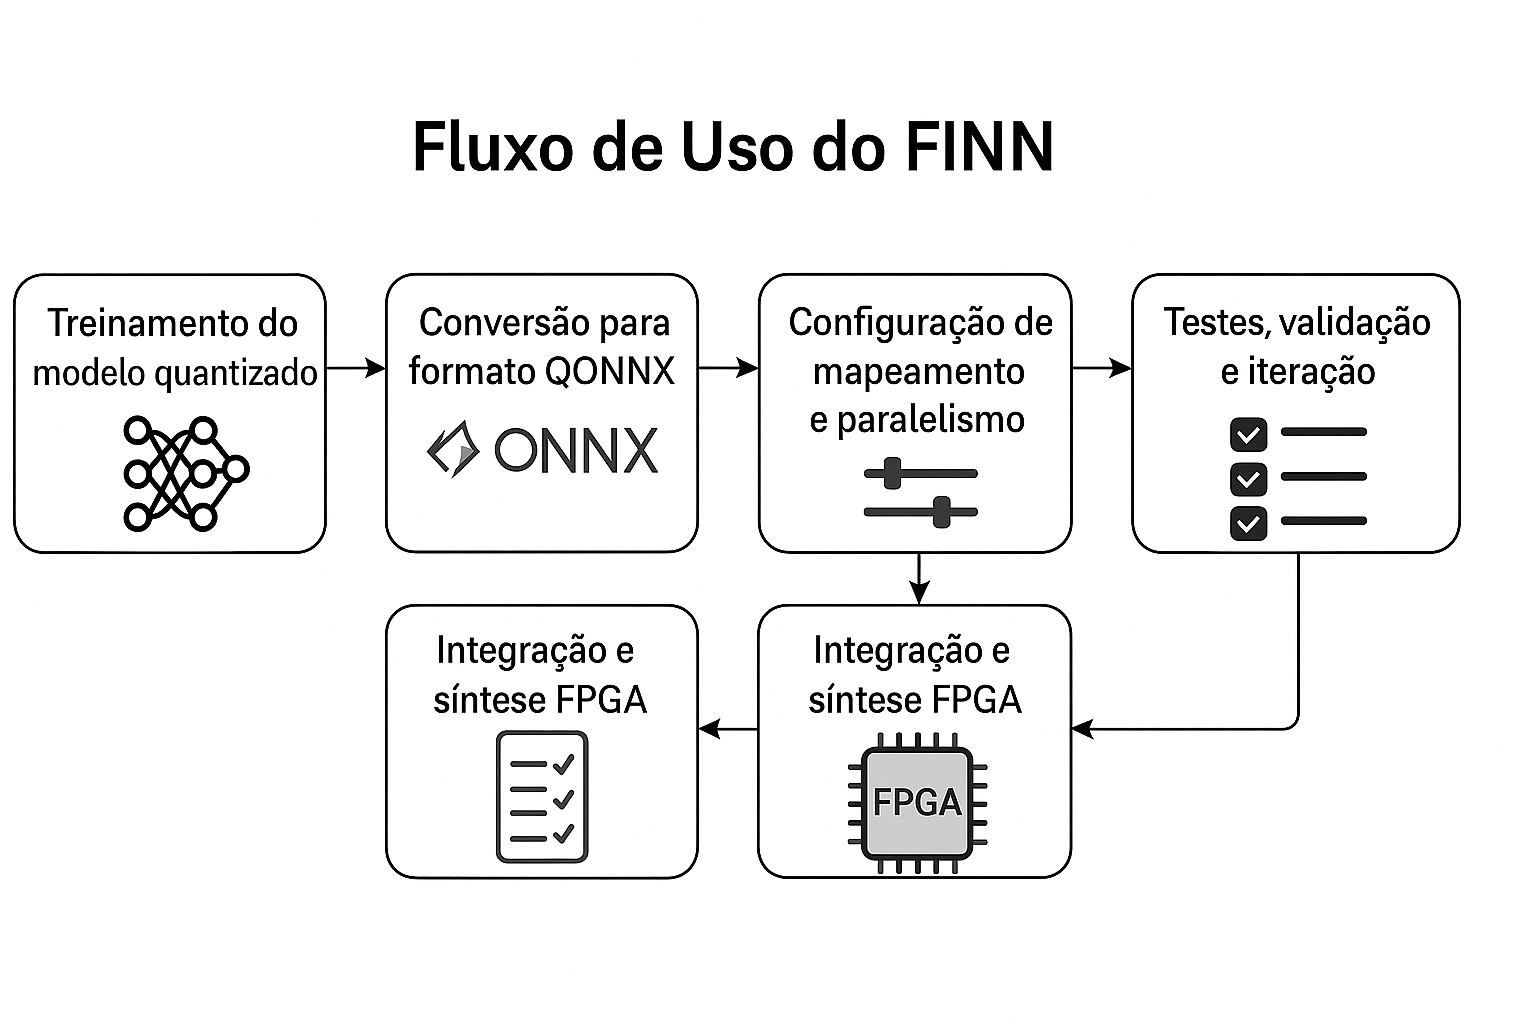
\includegraphics[width=0.80\linewidth]{FluxoUsoFINN.png}
%    \caption{Fluxo do uso do FINN. \\ Fonte: O autor.}
%    \label{fig:FINN_FluxoGeral}
%\end{figure}
%
%O processo se inicia com o \textbf{treinamento de um modelo quantizado}, normalmente conduzido no ambiente \textit{Brevitas}, onde pesos e ativações são ajustados para operar com baixa precisão (por exemplo, 1, 2, 4 ou 8 bits), mantendo a acurácia dentro de margens aceitáveis. Em seguida, o modelo é exportado no formato \textbf{QONNX} (\textit{Quantized Open Neural Network Exchange}), que atua como uma representação intermediária padronizada para a interoperabilidade entre frameworks de aprendizado e \mbox{ferramentas de síntese de hardware.}
%
%Na sequência, o usuário define os parâmetros de \textbf{mapeamento e paralelismo}, determinando a quantidade de unidades de computação, a profundidade de pipeline e o balanceamento entre latência e throughput. O \textbf{FINN Compiler} então converte o modelo quantizado em uma estrutura de hardware equivalente, gerando módulos em HLS ou RTL que representam cada camada da rede neural. Esses módulos são organizados em um fluxo contínuo de dados (\textit{dataflow architecture}), no qual as saídas de uma camada são transmitidas diretamente para a próxima, minimizando a necessidade \mbox{de armazenamento intermediário.}
%
%Após a \textbf{geração dos IPs} (blocos de hardware), o projeto é integrado em ambiente de síntese como o \textit{Vivado} ou o \textit{Vitis}, com conexão via barramento AXI e lógica de controle personalizada. A partir dessa integração, realiza-se a síntese, implementação e geração do \textbf{bitstream}, que configura o FPGA conforme o design projetado.
%
%Finalmente, a etapa de \textbf{teste e validação} avalia o desempenho real do sistema em termos de utilização de recursos, latência, consumo energético e acurácia. Esse processo é iterativo — ajustes finos podem ser aplicados para otimizar o desempenho, explorar paralelismo adicional ou adaptar o hardware a diferentes topologias de rede.
%
%Assim, o diagrama sintetiza o papel do FINN como um elo entre o domínio do aprendizado profundo e o projeto digital reconfigurável, demonstrando como a abstração de alto nível pode ser convertida, de forma automatizada e eficiente, em uma arquitetura física otimizada para execução em FPGA.
%
%
%O FINN também possui extensões importantes, como o \textbf{FINN-R}, um fluxo \textit{end-to-end} de exploração de espaço de design (\textit{Design Space Exploration}) que automatiza a análise de \textit{trade-offs} entre desempenho, consumo e área de hardware, gerando configurações otimizadas de aceleradores personalizados.
%
%Considerando sua capacidade de paralelismo massivo, determinismo temporal e eficiência energética, o FINN consolida-se como uma ferramenta de destaque para a execução de algoritmos de aprendizado profundo em tempo real. Essas características o tornam especialmente adequado para aplicações industriais e embarcadas, nas quais a confiabilidade, a baixa latência e a integração direta com sensores são requisitos fundamentais. Assim, compreender o fluxo de uso do FINN e sua arquitetura interna constitui um passo essencial para o desenvolvimento de sistemas inteligentes de monitoramento e diagnóstico baseados em FPGA.
%
%
%Na subseção seguinte, são apresentados estudos e trabalhos recentes que exploram o uso de FPGAs na aceleração de redes neurais e em aplicações de aprendizado de máquina, evidenciando o estado da arte e as tendências atuais dessa tecnologia no contexto da Inteligência Artificial embarcada.

%\subsection{Aplicações Recentes de FPGAs em Aprendizado de Máquina}
%
%\textcolor{red}{Ainda estou selecionado/lendo/resumindo os artigos}